\begin{exercise}
      {ID-fffc17cb928a23befe424d29a4c070d9d80648be}
      {Schulweg}
  \ifproblem\problem
    Zwei Kinder, die im selben Haus wohnen, gehen gemeinsam in die gleiche
    Schule. Das erste Kind geht die Hälfte der Zeit mit einer
    Durchschnittsgeschwindigkeit von \sikmh{5}, danach mit \sikm{4}. Das
    zweite Kind geht die Hälfte des Weges mit einer Durchschnittsgeschwindigkeit
    von \sikmh{4}, danach mit \sikmh{5}. Welches Kind erreicht die Schule
    zuerst?
  \fi
  \ifoutline\outline
    Angenommen, das erste Kind bräuchte zwei Stunden bis in die Schule:
    Wie weit ist dann der Schulweg, und wie lange wäre das andere Kind unterwegs?
  \fi
  \ifoutcome\outcome
    \begin{center}
      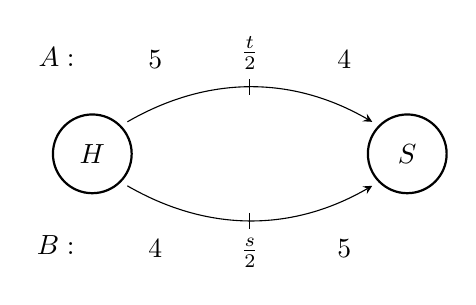
\begin{tikzpicture}
        \coordinate (A)  at (0, 0);
        \coordinate (B)  at (4, 0);
        \coordinate (An) at (45:5mm);
        \coordinate (As) at (315:5mm);
        \coordinate (Bn) at ([shift={(4, 0)}]135:5mm);
        \coordinate (Bs) at ([shift={(4, 0)}]225:5mm);
        \node at (A) {$H$};
        \node at (B) {$S$};
        \draw[line width=0.8pt] (A) circle[radius=5mm];
        \draw[line width=0.8pt] (B) circle[radius=5mm];
        \draw[shorten <=3pt, shorten >=3pt, ->, >=stealth] (An) to[out=30, in=150] (Bn);
        \draw[shorten <=3pt, shorten >=3pt, ->, >=stealth] (As) to[out=330, in=210] (Bs);
        \draw (2,  0.75) -- (2,  0.95) node[above]{$\frac{t}{2}$};
        \draw (2, -0.75) -- (2, -0.95) node[below]{$\frac{s}{2}$};
        \node at (0.8, 1.2) {\sikmh{5}};
        \node at (3.2, 1.2) {\sikmh{4}};
        \node at (0.8, -1.2) {\sikmh{4}};
        \node at (3.2, -1.2) {\sikmh{5}};
        \node[left=1mm] at (0,  1.23) {$A:$};
        \node[left=1mm] at (0, -1.16) {$B:$};
      \end{tikzpicture}
    \end{center}
    Wenn man annimmt, dass das erste Kind für den Schulweg $t_{A}$ Stunden benötigt,
    dann ergibt sich folgende Länge für den Schulweg:
    \begin{equation*}
      \frac{t_{A}}{2}\cdot5+\frac{t_{A}}{2}\cdot4
      =
      \frac{9\cdot t_{A}}{2}
      \quad\text{(in \si{\kilo\metre})}
    \end{equation*}

    Diese Strecke legt das zweite Kind in folgender Zeit zurück:
    \begin{equation*}
      \left.
      \begin{array}{lcl}
        \displaystyle\frac{9\cdot t_{A}}{4}=t_{B1}\cdot4 & \Rightarrow & t_{B1}=\displaystyle\frac{9}{16}t_{A}\\[3ex]
        \displaystyle\frac{9\cdot t_{A}}{4}=t_{B2}\cdot5 & \Rightarrow & t_{B2}=\displaystyle\frac{9}{20}t_{A}
      \end{array}
      \quad\right\}
      \quad\Rightarrow\quad
      t_{B}=\left(\frac{45}{80}+\frac{36}{80}\right)\cdot t_{A}=\frac{81}{80}\cdot t_{A}
    \end{equation*}

    Das erste Kind erreicht die Schule also früher.
  \fi
\end{exercise}
